\chapter{Funcionamento do sistema}

Nesta seção estão dispostas as funcionalidades e interfaces desenvolvidas ao longo do projeto.

\section{Firmware para controle do módulo WIFI}

Foi utilizado um microcontrolador fabricado pela empresa Espressif o ESP8266, este microcontrolador é controlado por um \textit{firmware} escrito utilizando o \textit{framework} Arduíno. Este framework divide-se em duas partes, seu núcleo, com as funções básicas de controle do hardware e uma lista de bibliotecas que permitem a expansão e o acesso a novos periféricos de outros modelos de placas micro controladas, como a ESP8266 que possui uma interface de comunicação via WIFI. Através desta interface de rede WIFI, são efetuadas as trocas de mensagens via TCP com a central de controle, utilizando o protocolo de comunicação MQTT, a responsabilidade da central de controle é de fazer o gerenciamento de dispositivos conectados na rede e a distribuição de mensagens.

Na central de controle um serviço de controle de mensagens, chamado \textit{broker} de mensagens, recebe e envia mensagens ela é uma camada intermediária entre os Módulos Auxiliares (controlados pelo ESP8266) e as ações que o usuário deseja fazer, de um lado esta central sabe "conversar" com os módulos, de outro utilizando a API para controle ela troca mensagens com o usuário.

\section{API para controle de Hardware}

Esta API é o caminho pelo qual aplicativos variados podem se comunicar com a ponta final do sistema, os Módulos Auxiliares. Para que um aplicativo possa utiliza-la, basta que este consiga consumir uma API RESt, esta é uma forma de tornar este sistema atrativo para outros desenvolvedores que tenham interesse em fazer algum tipo de integração com um sistema de domótica simplificado como é o Ysto.

Esta API é a Figura central do sistema, todas as ações e controles de comportamento do sistema passam por ela. As sub-seções a seguir descrevem de forma mais detalhada seu funcionamento.

\subsection{Sobre esta API}
Este \textit{end-point} traz informações sobre a API, dados como nome e versão. A Figura \ref{api-about} monstra esta chamada através de um cliente de RESt genérico.

\begin{figure}[H]
\caption{\label{api-about} Informações da API}
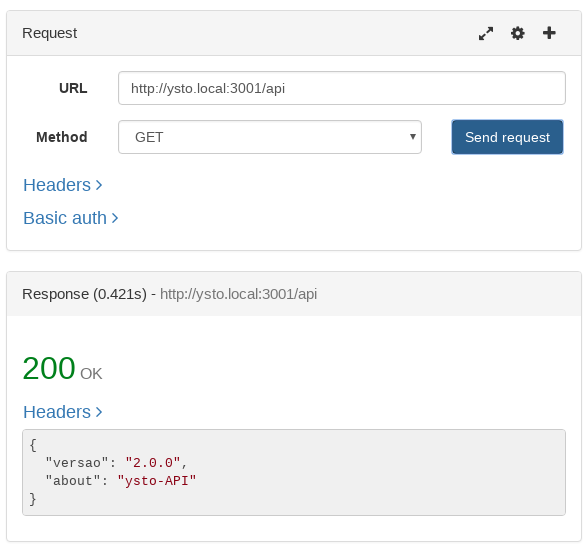
\includegraphics[scale=0.35]{img/05-api-about.png}
\legend{Fonte: Autor do projeto}
\end{figure}

\subsection{Solicitação de token}
Este \textit{end-point} espera o envio das credenciais de um usuário válido para então devolver um token de segurança, por motivo de simplificação este token não possui um tempo de validade, ficando a critério do desenvolvedor elaborar uma politica para lidar com a validade deste token, uma boa prática seria armazenar este token no que a World Wide Web Consortium (W3C) chama de \textit{session storage}, desta forma o token existe apenas no tempo de "vida" da janela do aplicativo. A Figura \ref{api-auth} mostra o envio de credenciais e o recebimento de um token válido.

\begin{figure}[H]
\caption{\label{api-auth} Requisição de token de acesso}
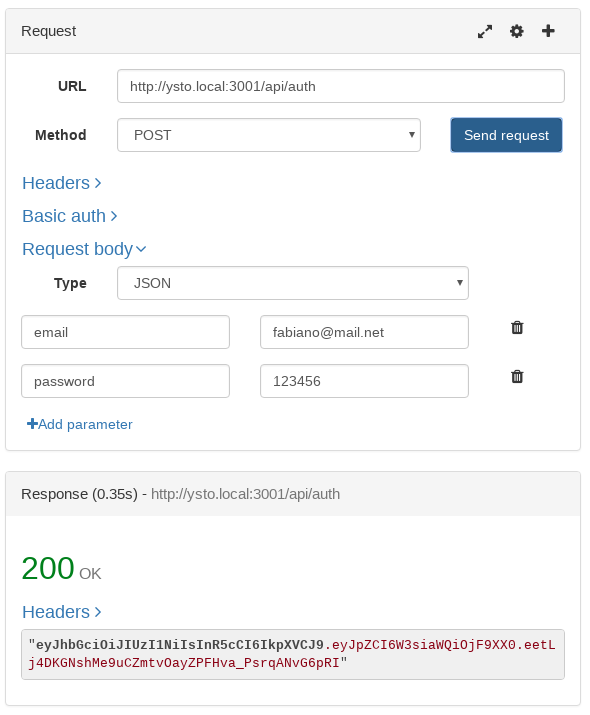
\includegraphics[scale=0.35]{img/06-api-auth.png}
\legend{Fonte: Autor do projeto}
\end{figure}

\subsection{Manutenção de usuários do sistema}
Este \textit{end-point} faz as operações de CRUD dos usuários do sistema, a idéia é que o banco seja criado com um usuário padrão e a partir deste usuário todas as ações relacionadas a usuários sejam feitas a partir dele, conforme a necessidade dos moradores. Este é um \textit{end-point} que exige um token de autenticação válido no cabeçalho da mensagem, solicitações que não possuem esta assinatura serão recusadas pela central de controle, a Figura \ref{api-users} mostra o cadastro de um usuário via API.

\begin{figure}[H]
\caption{\label{api-users} Manutenção de usuários}
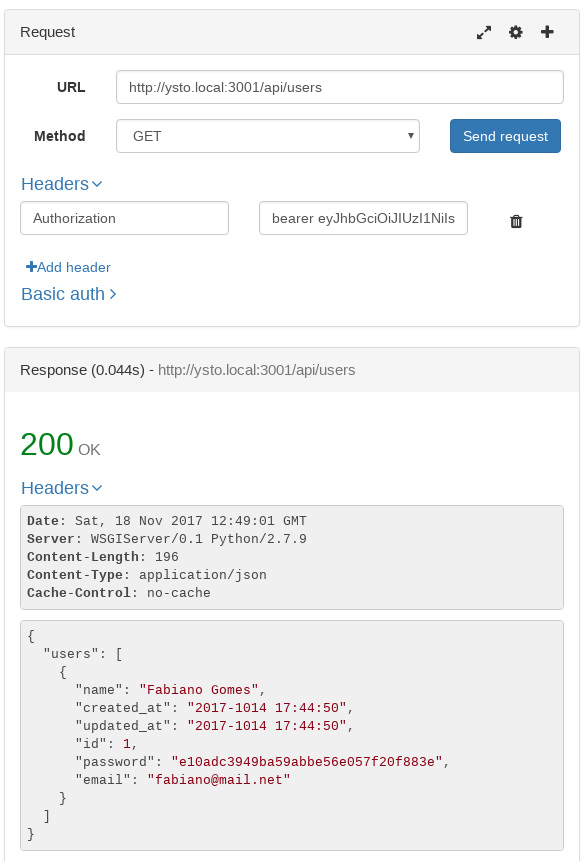
\includegraphics[scale=0.35]{img/07-api-users.png}
\legend{Fonte: Autor do projeto}
\end{figure}

\subsection{Manutenção de dispositivos do sistema}
Este \textit{end-point} faz as operações de CRUD de dispositivos que são controlados pelo sistema, é importante entender que esta é uma ação que deve estar integrada com o \textit{firmware} de controle dos Módulos Auxiliares, ou seja, o \textit{firmware} deve ser gravado com o mesmo tópico cadastrado na API. Atualmente a API controla apenas um tópico chamado relay, desta forma uma mensagem será endereçada da seguinte forma, tópico de destino <NOME-DISPOSITIVO>/output e conteúdo da mensagem [1 | 0] para ligar ou desligar a saída do módulo referenciado. A Figura \ref{api-devices} mostra como é feito o cadastro de um dispositivo, este \textit{ed-point} da API só aceita solicitações mediante um token válido.

\begin{figure}[H]
\caption{\label{api-devices} Manutenção de dispositivos}
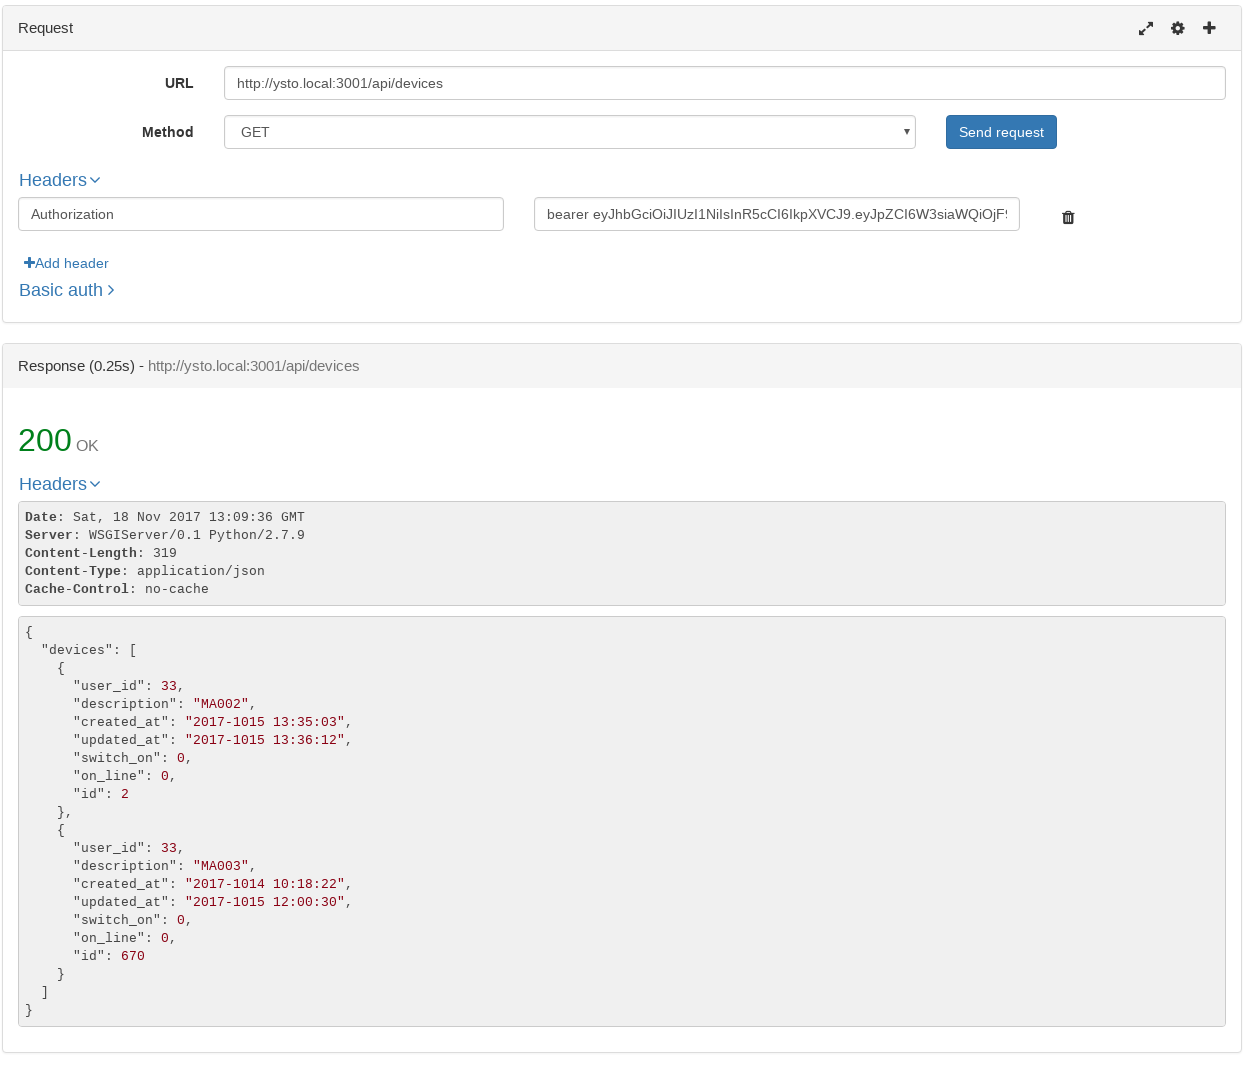
\includegraphics[scale=0.30]{img/08-api-devices.png}
\legend{Fonte: Autor do projeto}
\end{figure}

\subsection{Controle de dispositivo}
Este \textit{end-point} faz o controle de acionamento dos dispositivos cadastrados, ele recebe o comando de acionamento (ligar ou desligar) e repassa para o \textit{broker}, este por sua vez faz o envio para o Módulo Auxiliar correspondente, a Figura \ref{api-update-device} mostra este envio. Da mesma forma que os demais tópicos, este depende da assinatura por um token válido.

\begin{figure}[H]
\caption{\label{api-update-device} Atualização de estado de um dispositivo}
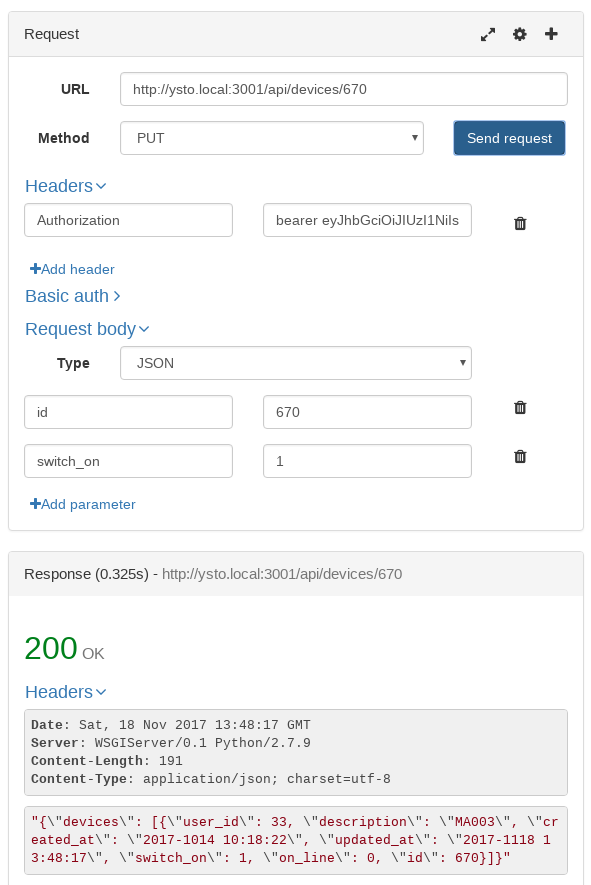
\includegraphics[scale=0.35]{img/09-update-device.png}
\legend{Fonte: Autor do projeto}
\end{figure}


\section{Interface Gráfica para controle do sistema}
Esta interface é um exemplo de como a API pode ser utilizada, fica hospedada na central de controle e pode ser acessada via \textit{web browser} por dispositivos móveis e \textit{desktops} independente do sistema operacional.

\subsection{Acesso ao sistema}
Na tela de acesso, Figura \ref{ui-login}, deve ser fornecido um email de usuário válido e sua senha.

\begin{figure}[H]
\caption{\label{ui-login} Tela de login}
\tcbox{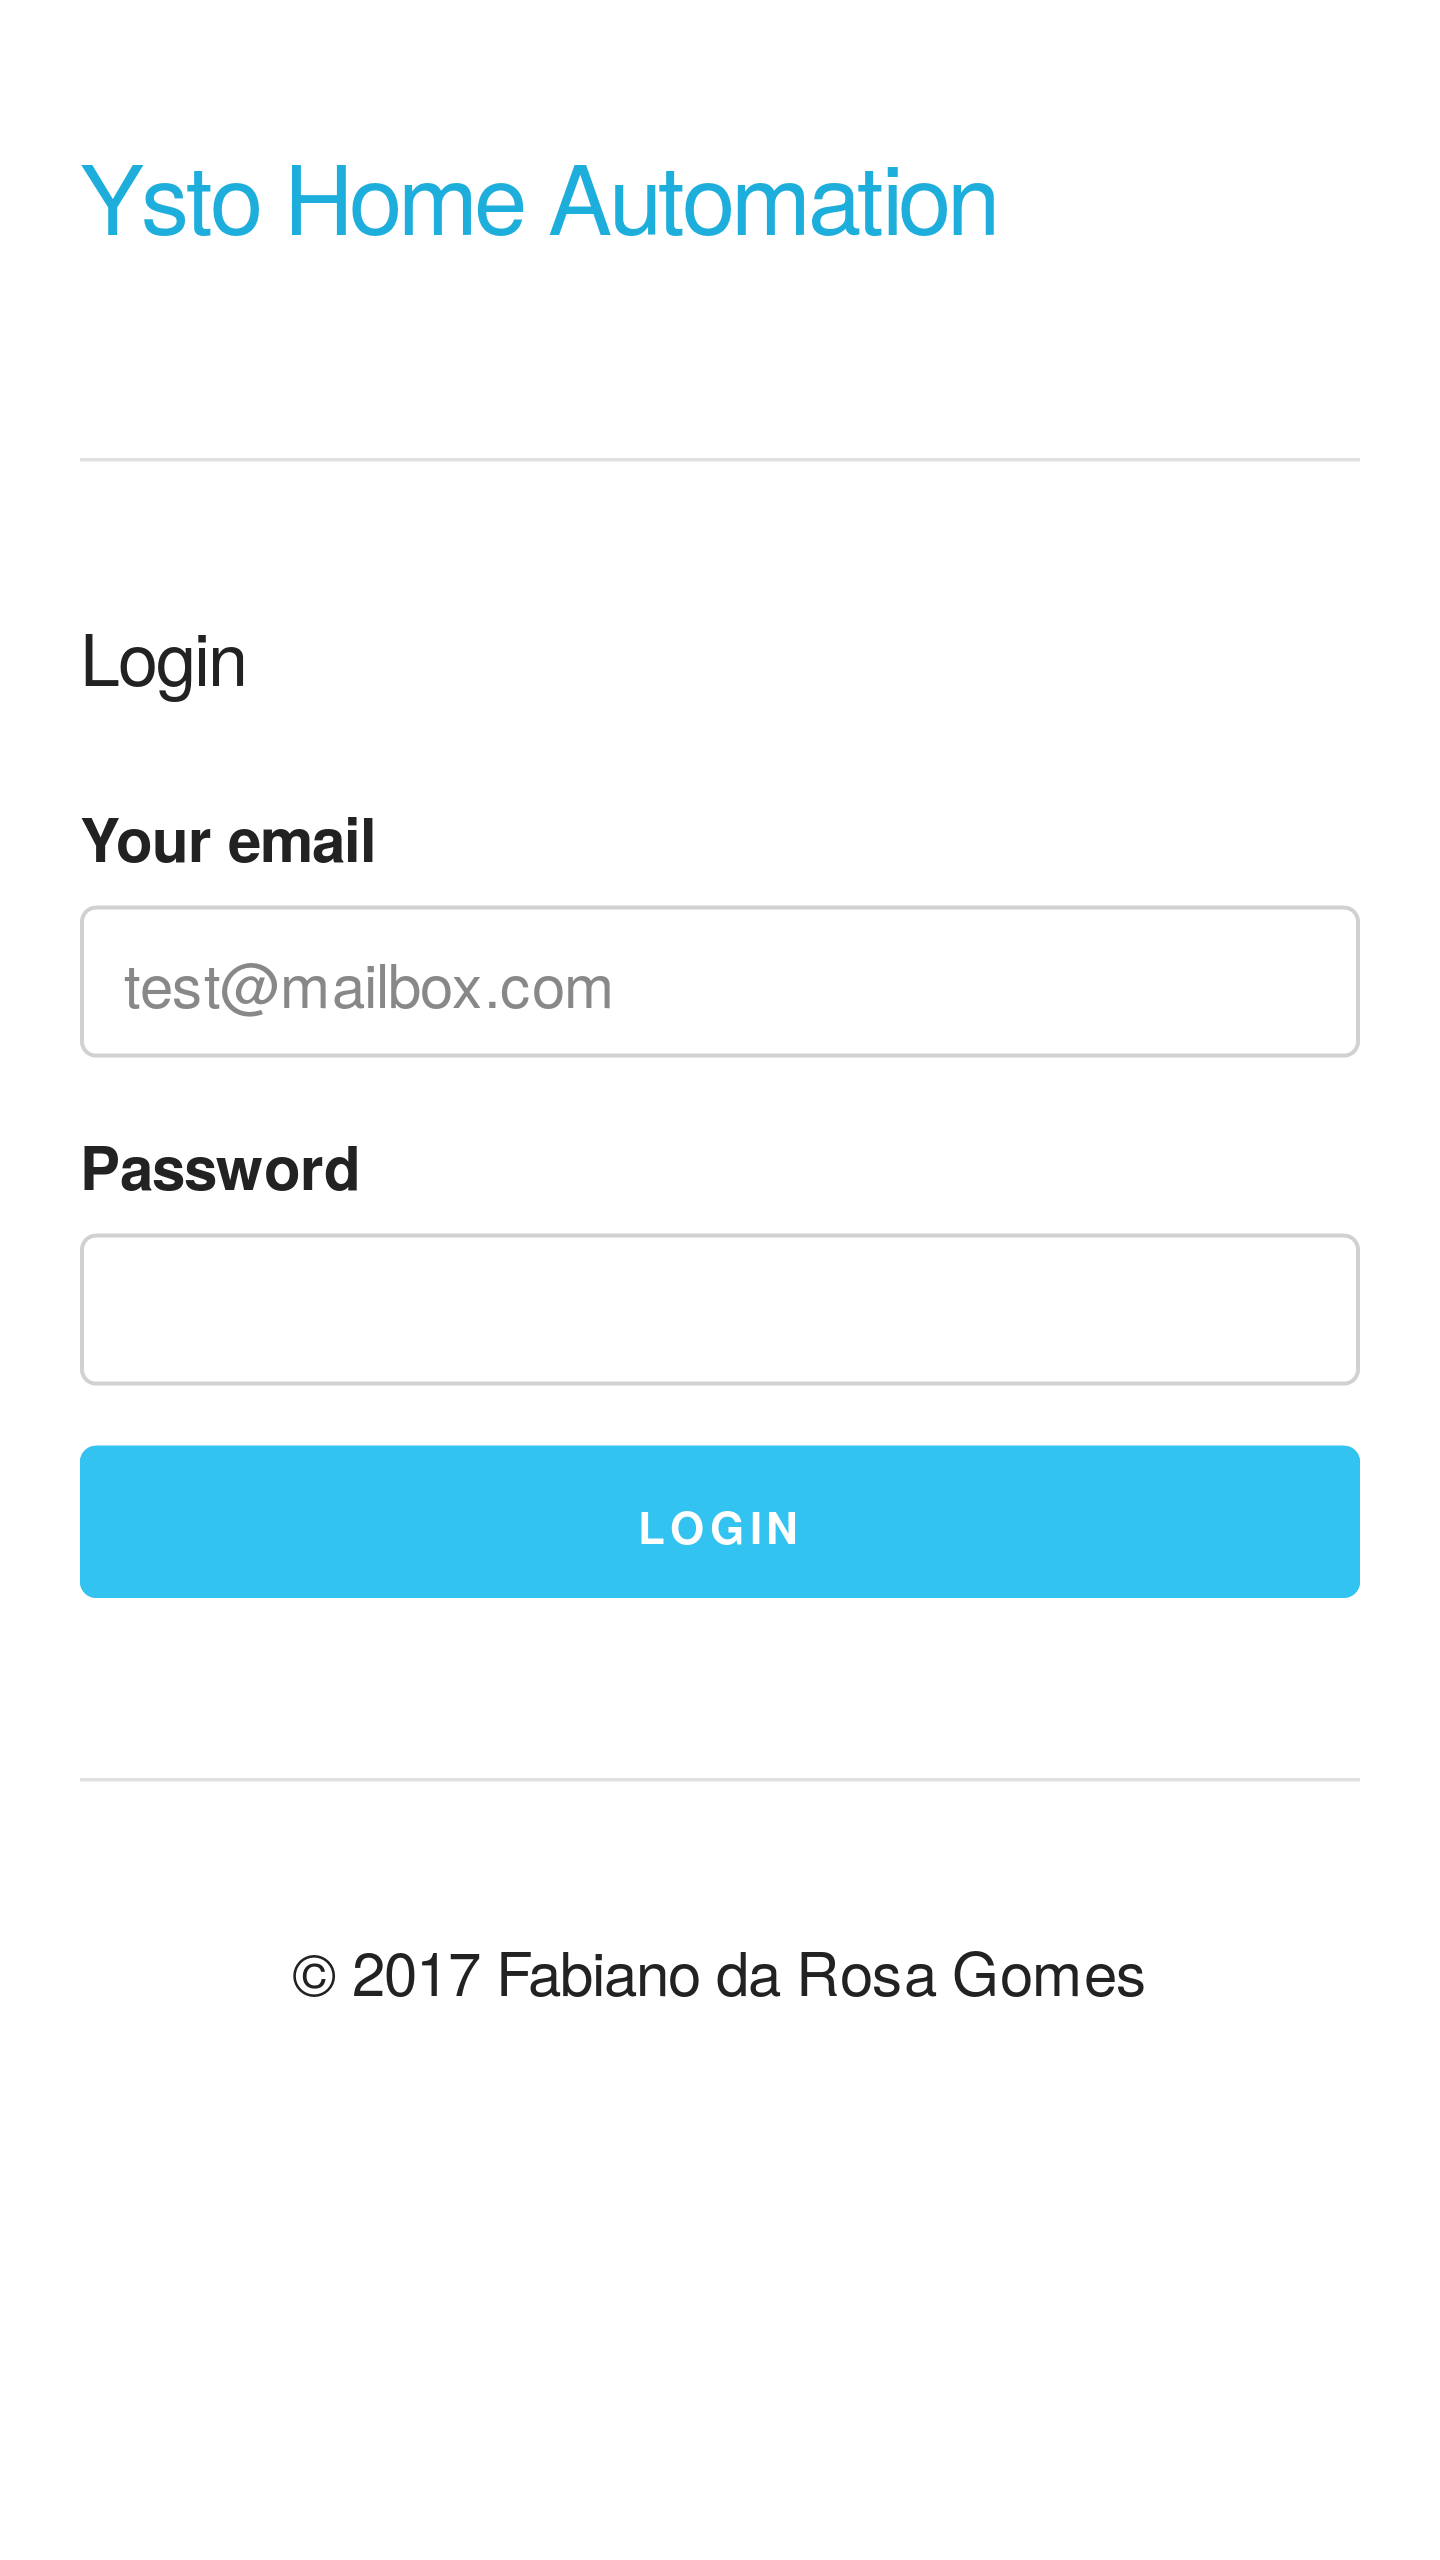
\includegraphics[scale=0.11]{img/00-login.png}}
\legend{Fonte: Autor do projeto}
\end{figure}

\subsection{Painel de controle}
No painel de controle é oferecido uma lista de possibilidades para o usuário navegar no sistema, a Figura \ref{ui-dashboard} mostra estas possibilidades.

\begin{figure}[H]
\caption{\label{ui-dashboard} Tela do painel de controle}
\tcbox{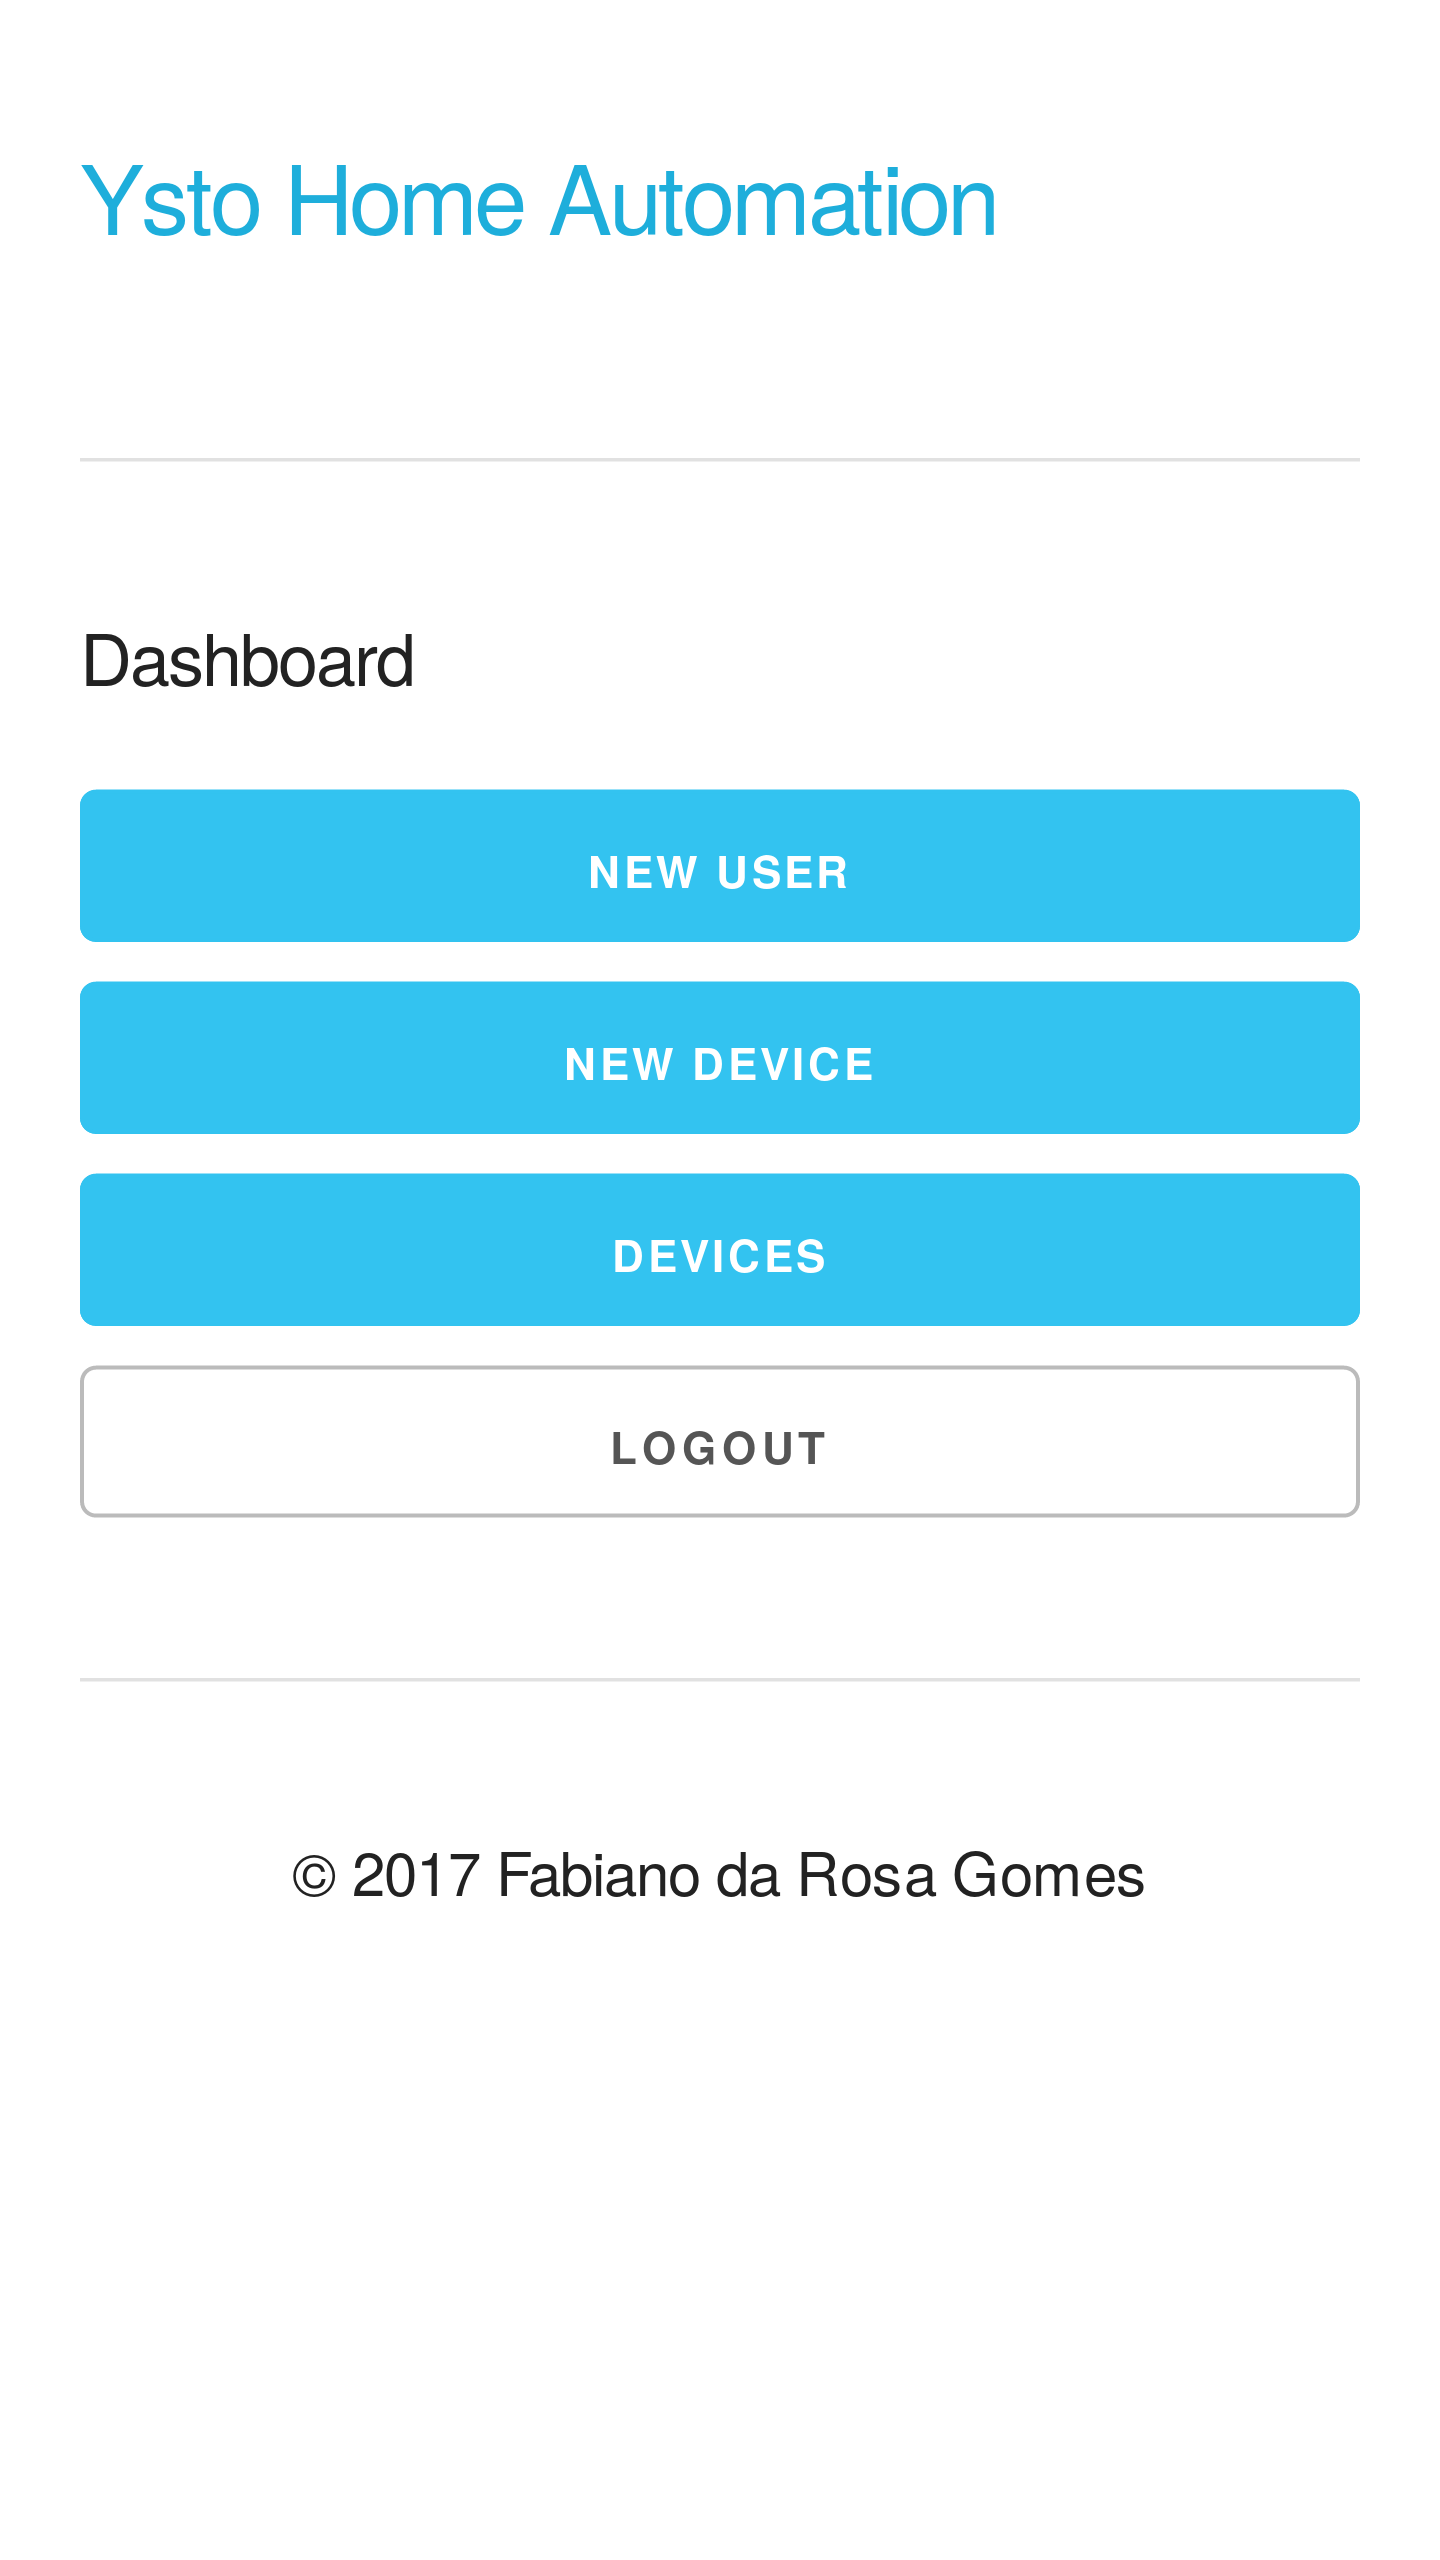
\includegraphics[scale=0.11]{img/01-dashboard.png}}
\legend{Fonte: Autor do projeto}
\end{figure}

\subsection{Cadastro de novos usuários}
Esta funcionalidade faz o cadastro de um novo usuário do sistema, utilizando uma email válido e a senha definida pelo usuário, apenas um \textit{hash} MD5 é armazenado no banco de dados. A Figura \ref{ui-new-user} mostra como é esta interface.

\begin{figure}[H]
\caption{\label{ui-new-user} Tela de cadastro de novos usuários}
\tcbox{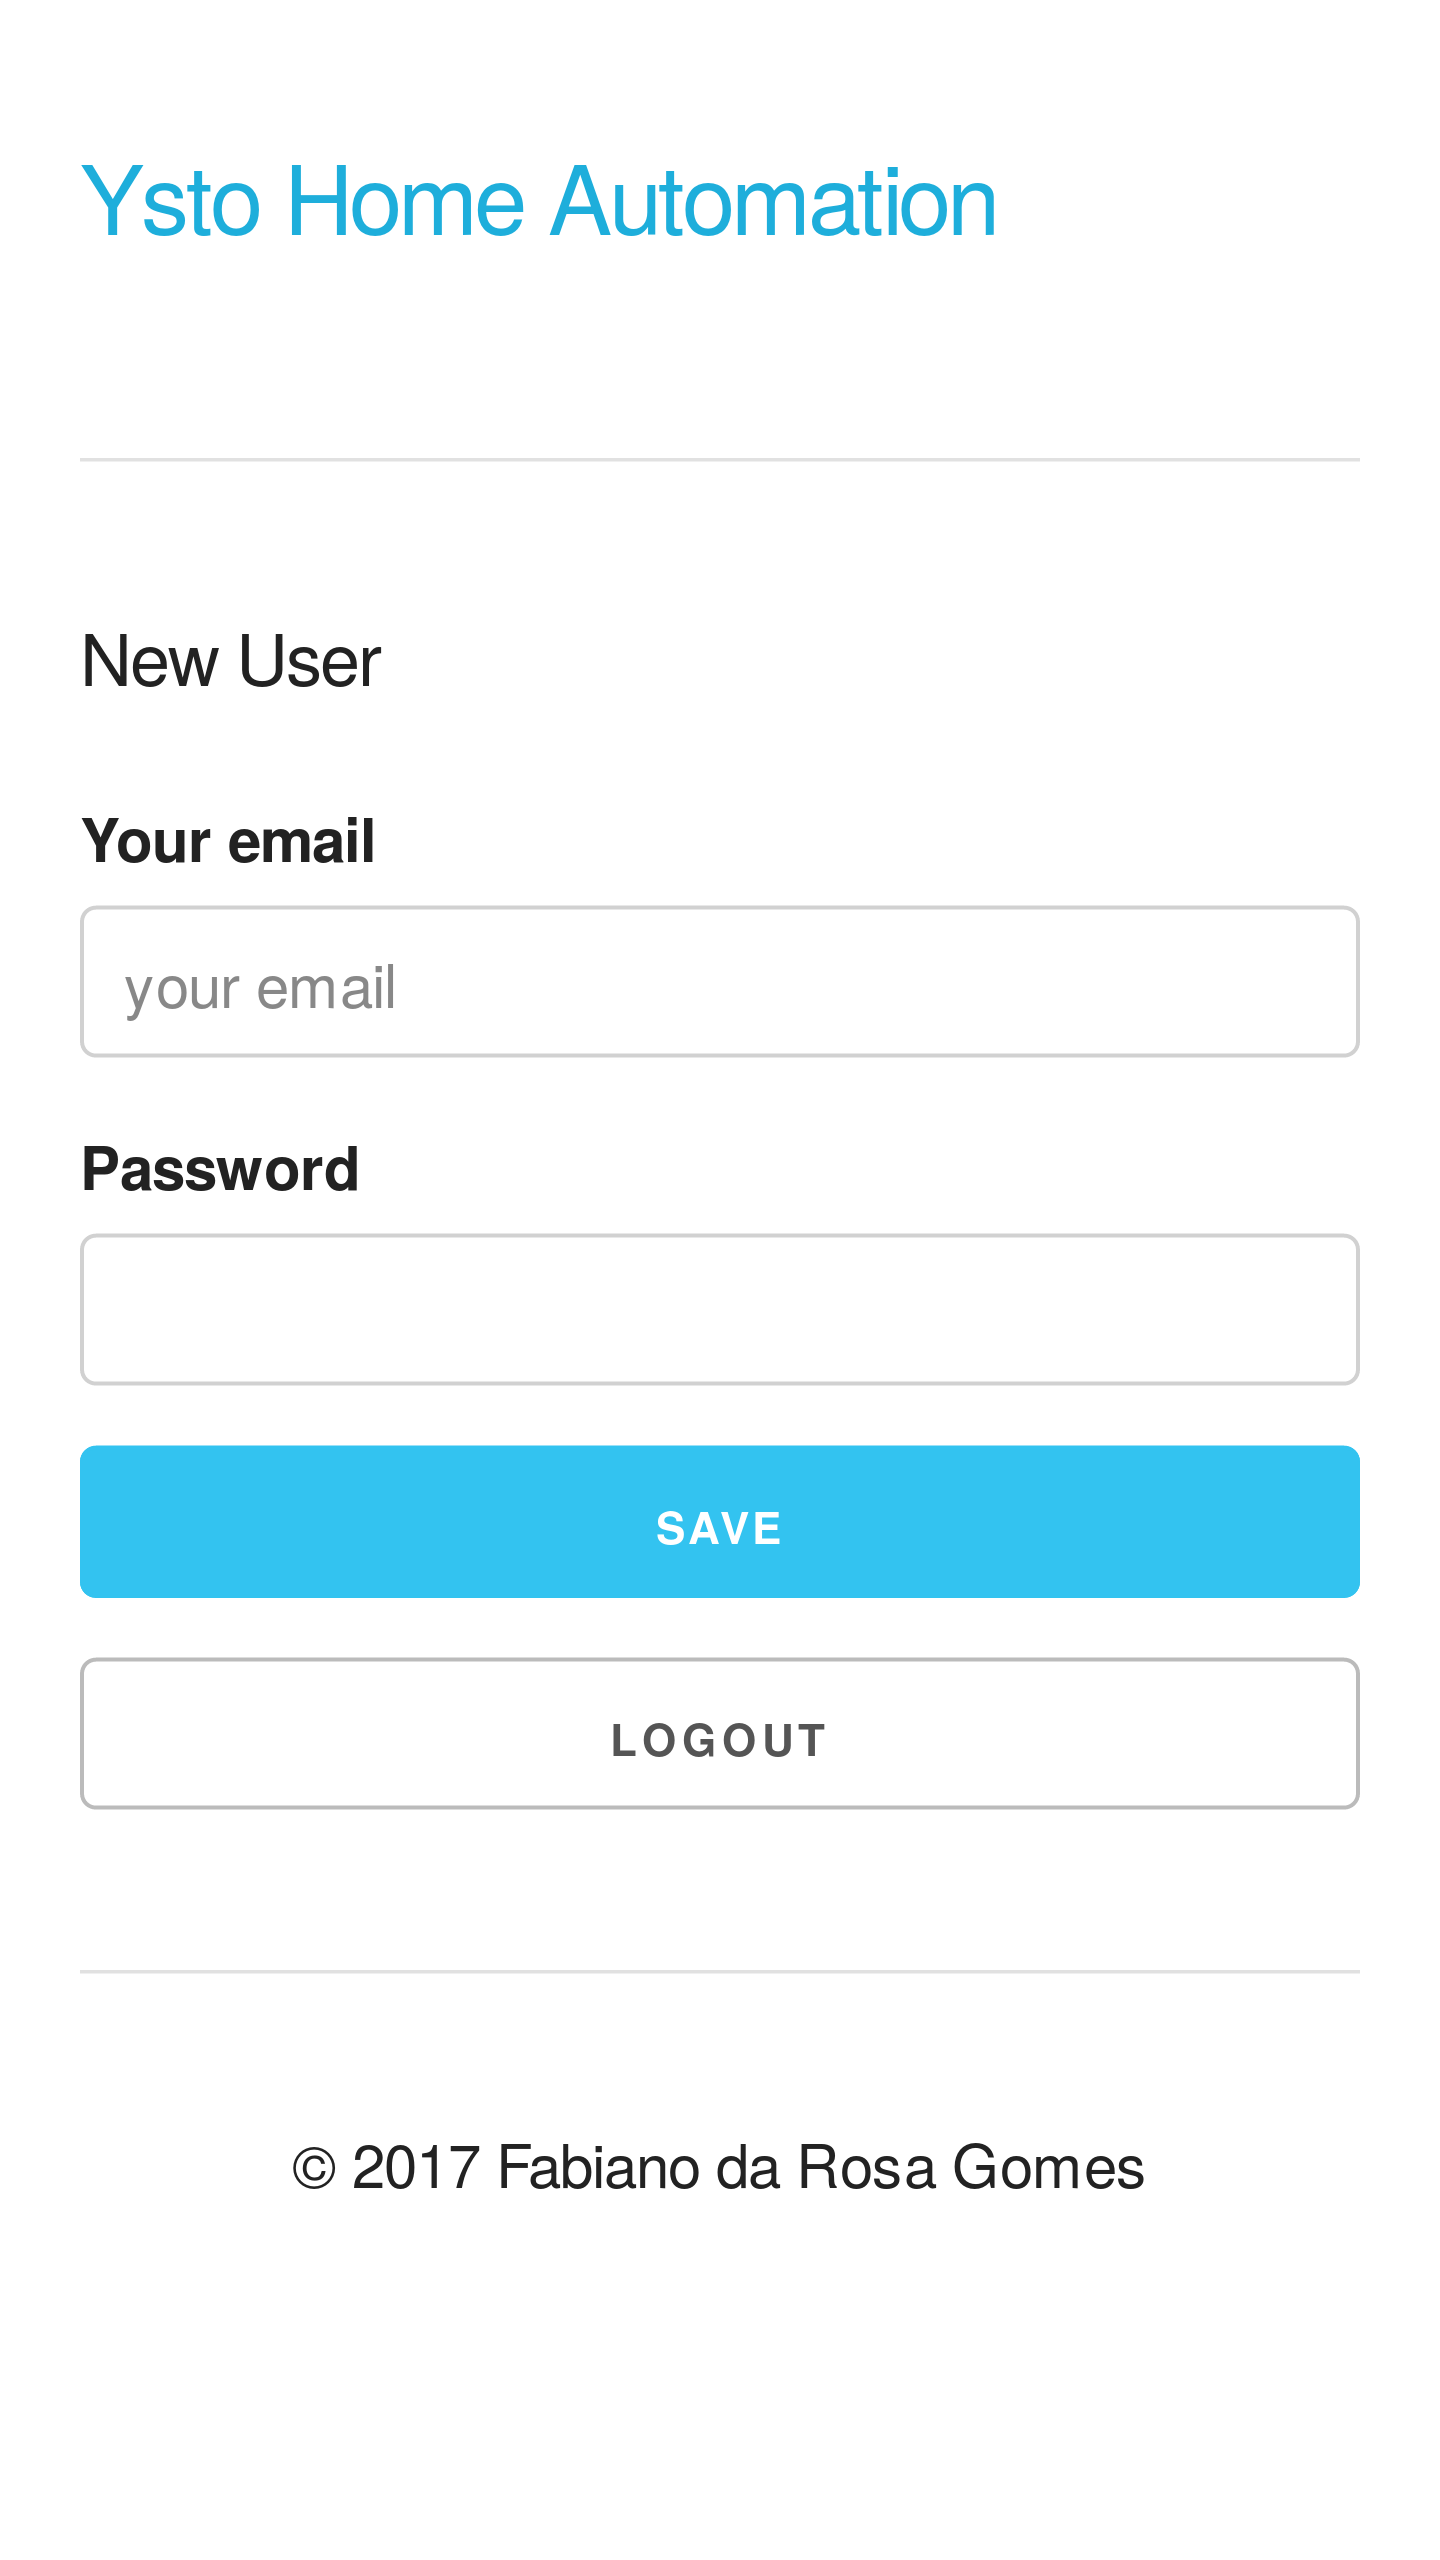
\includegraphics[scale=0.11]{img/02-new-user.png}}
\legend{Fonte: Autor do projeto}
\end{figure}

\subsection{Cadastro de novos dispositivos}
Esta funcionalidade faz o cadastro de novos dispositivos no sistema, importante lembrar que este nome deve ser o mesmo que é gravado no \textit{firmware} dos módulos de controle. A Figura \ref{ui-new-device} mostra esta funcionalidade.

\begin{figure}[H]
\caption{\label{ui-new-device} Tela de cadastro de novos dispositivos}
\tcbox{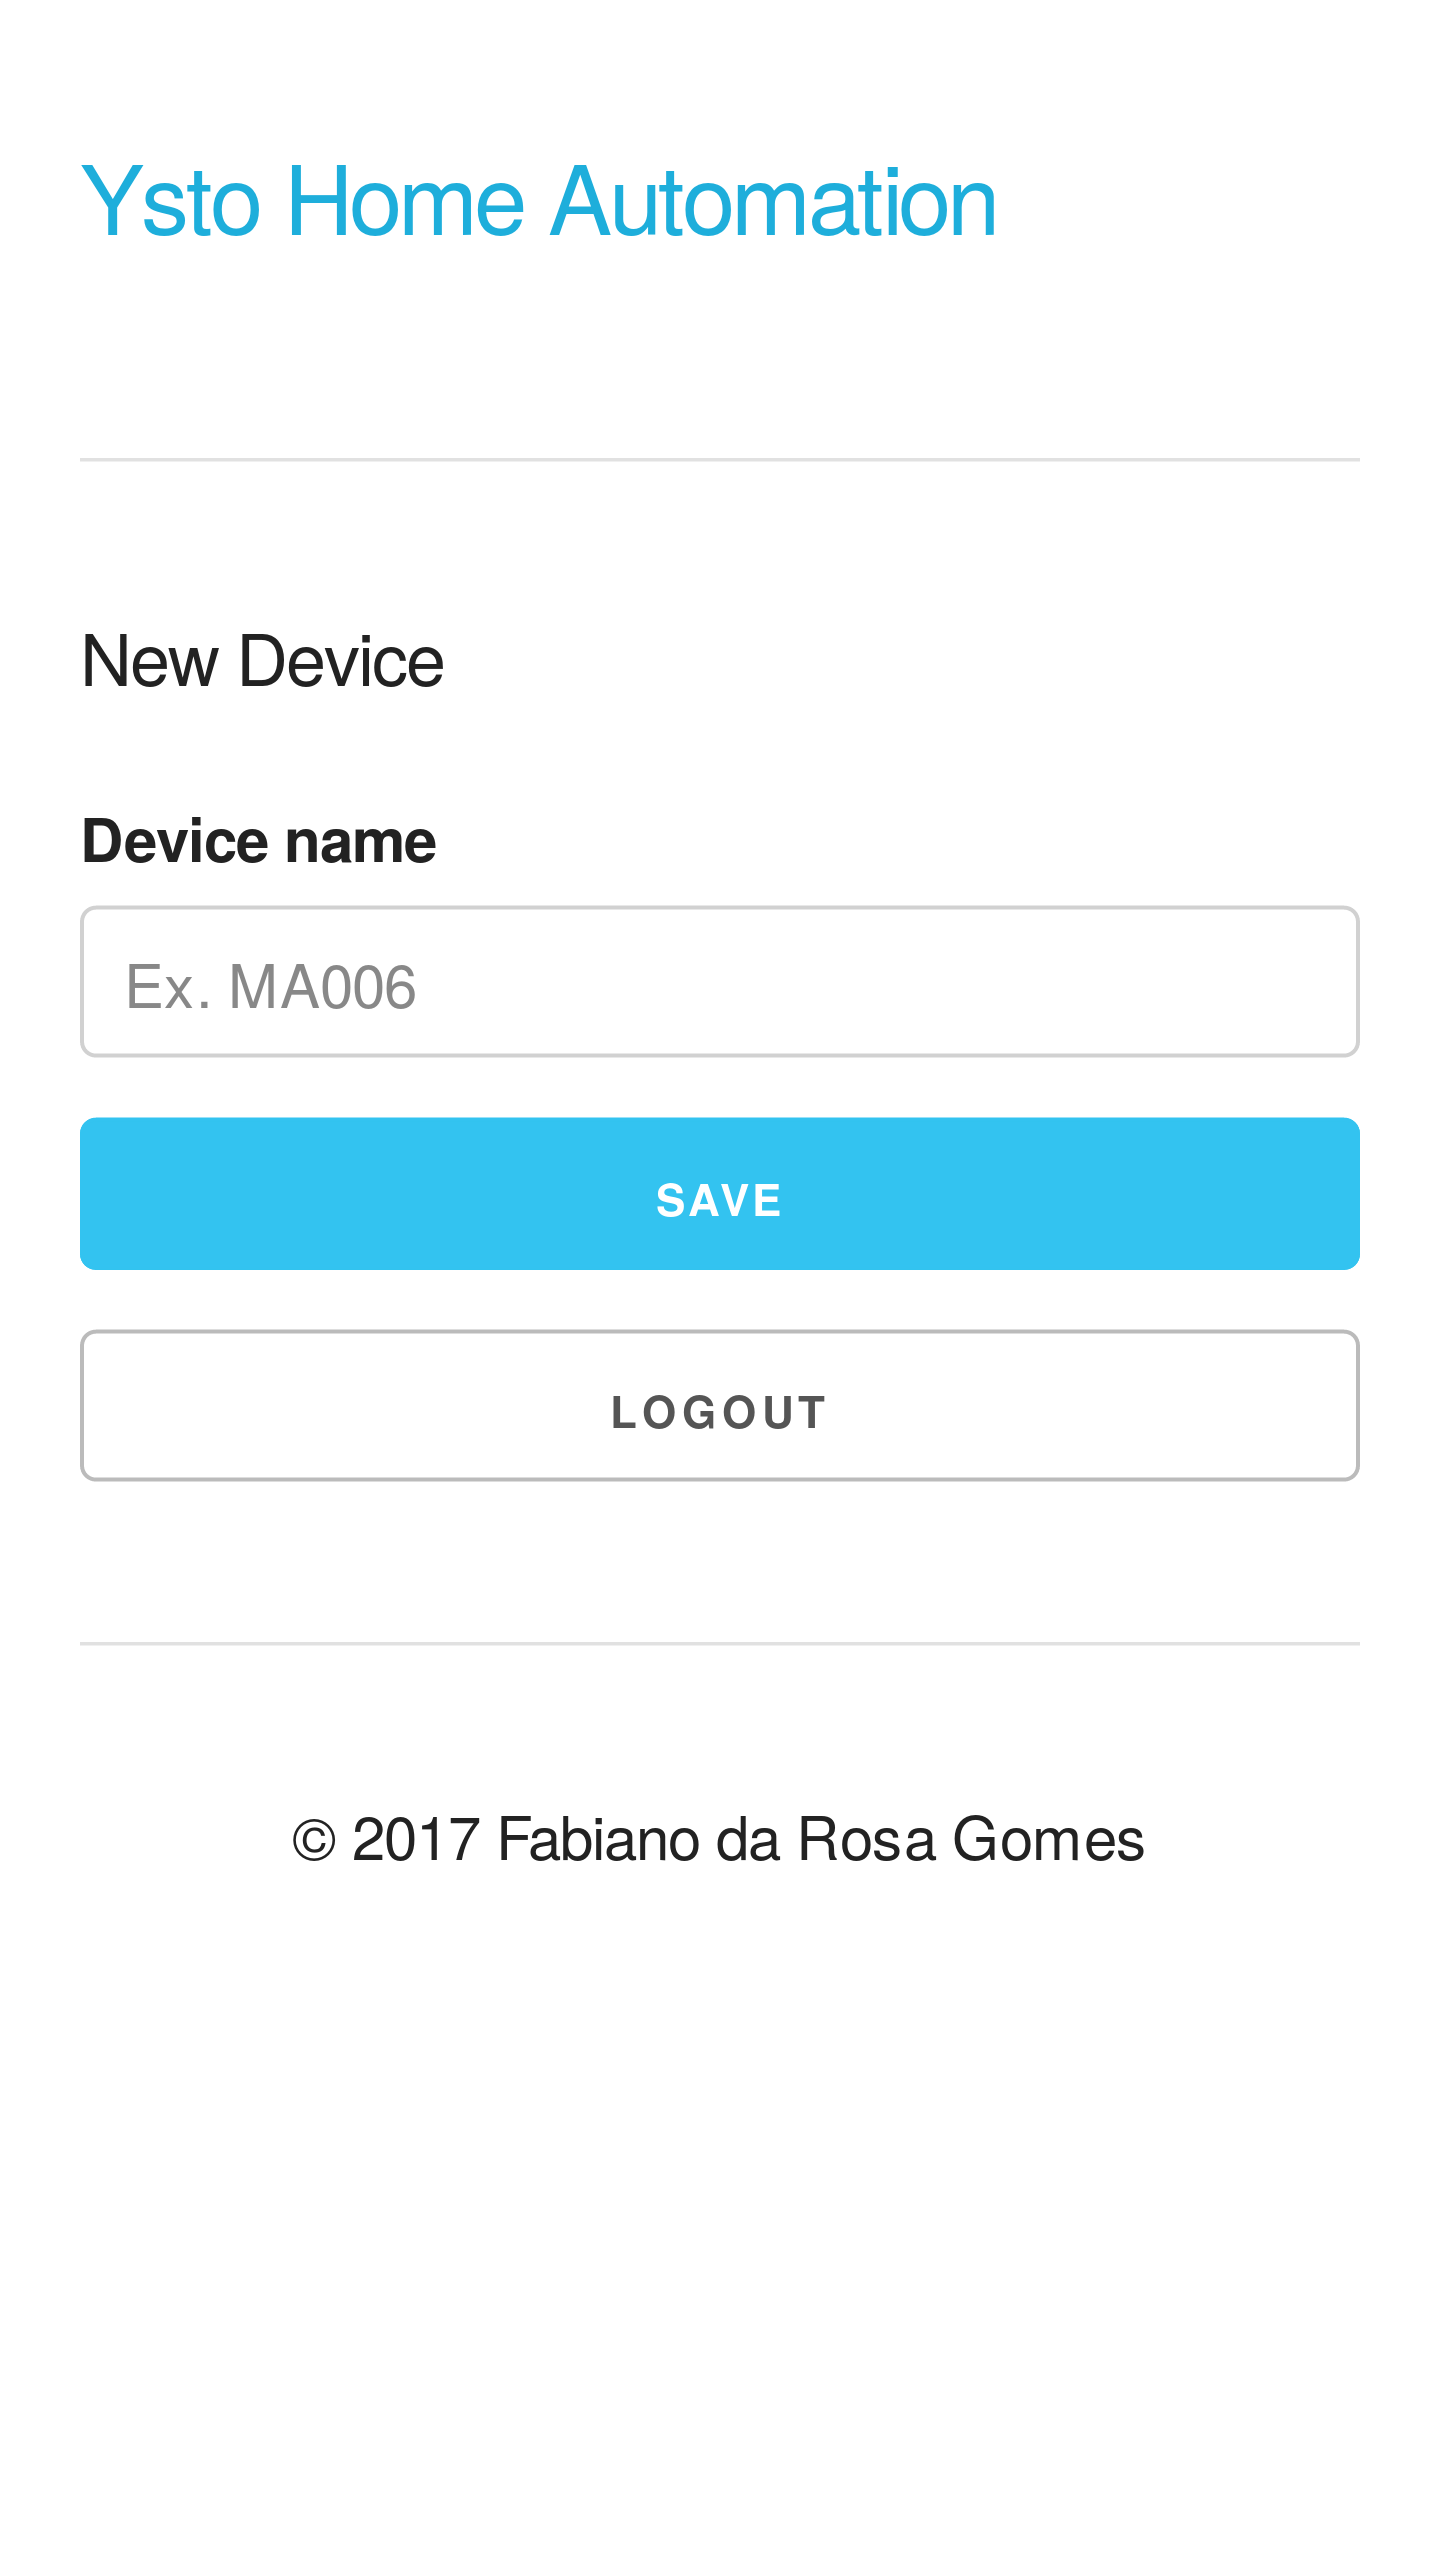
\includegraphics[scale=0.11]{img/03-new-device.png}}
\legend{Fonte: Autor do projeto}
\end{figure}

\subsection{Controle de dispositivos}
Nesta tela é apresentado a lista de dispositivos cadastrados é possível fazer a troca de estado utilizando o botão \textit{switch}, a Figura \ref{ui-handle-device} mostra como ficou esta tela.

\begin{figure}[H]
\caption{\label{ui-handle-device} Tela de controle dos dispositivos}
\tcbox{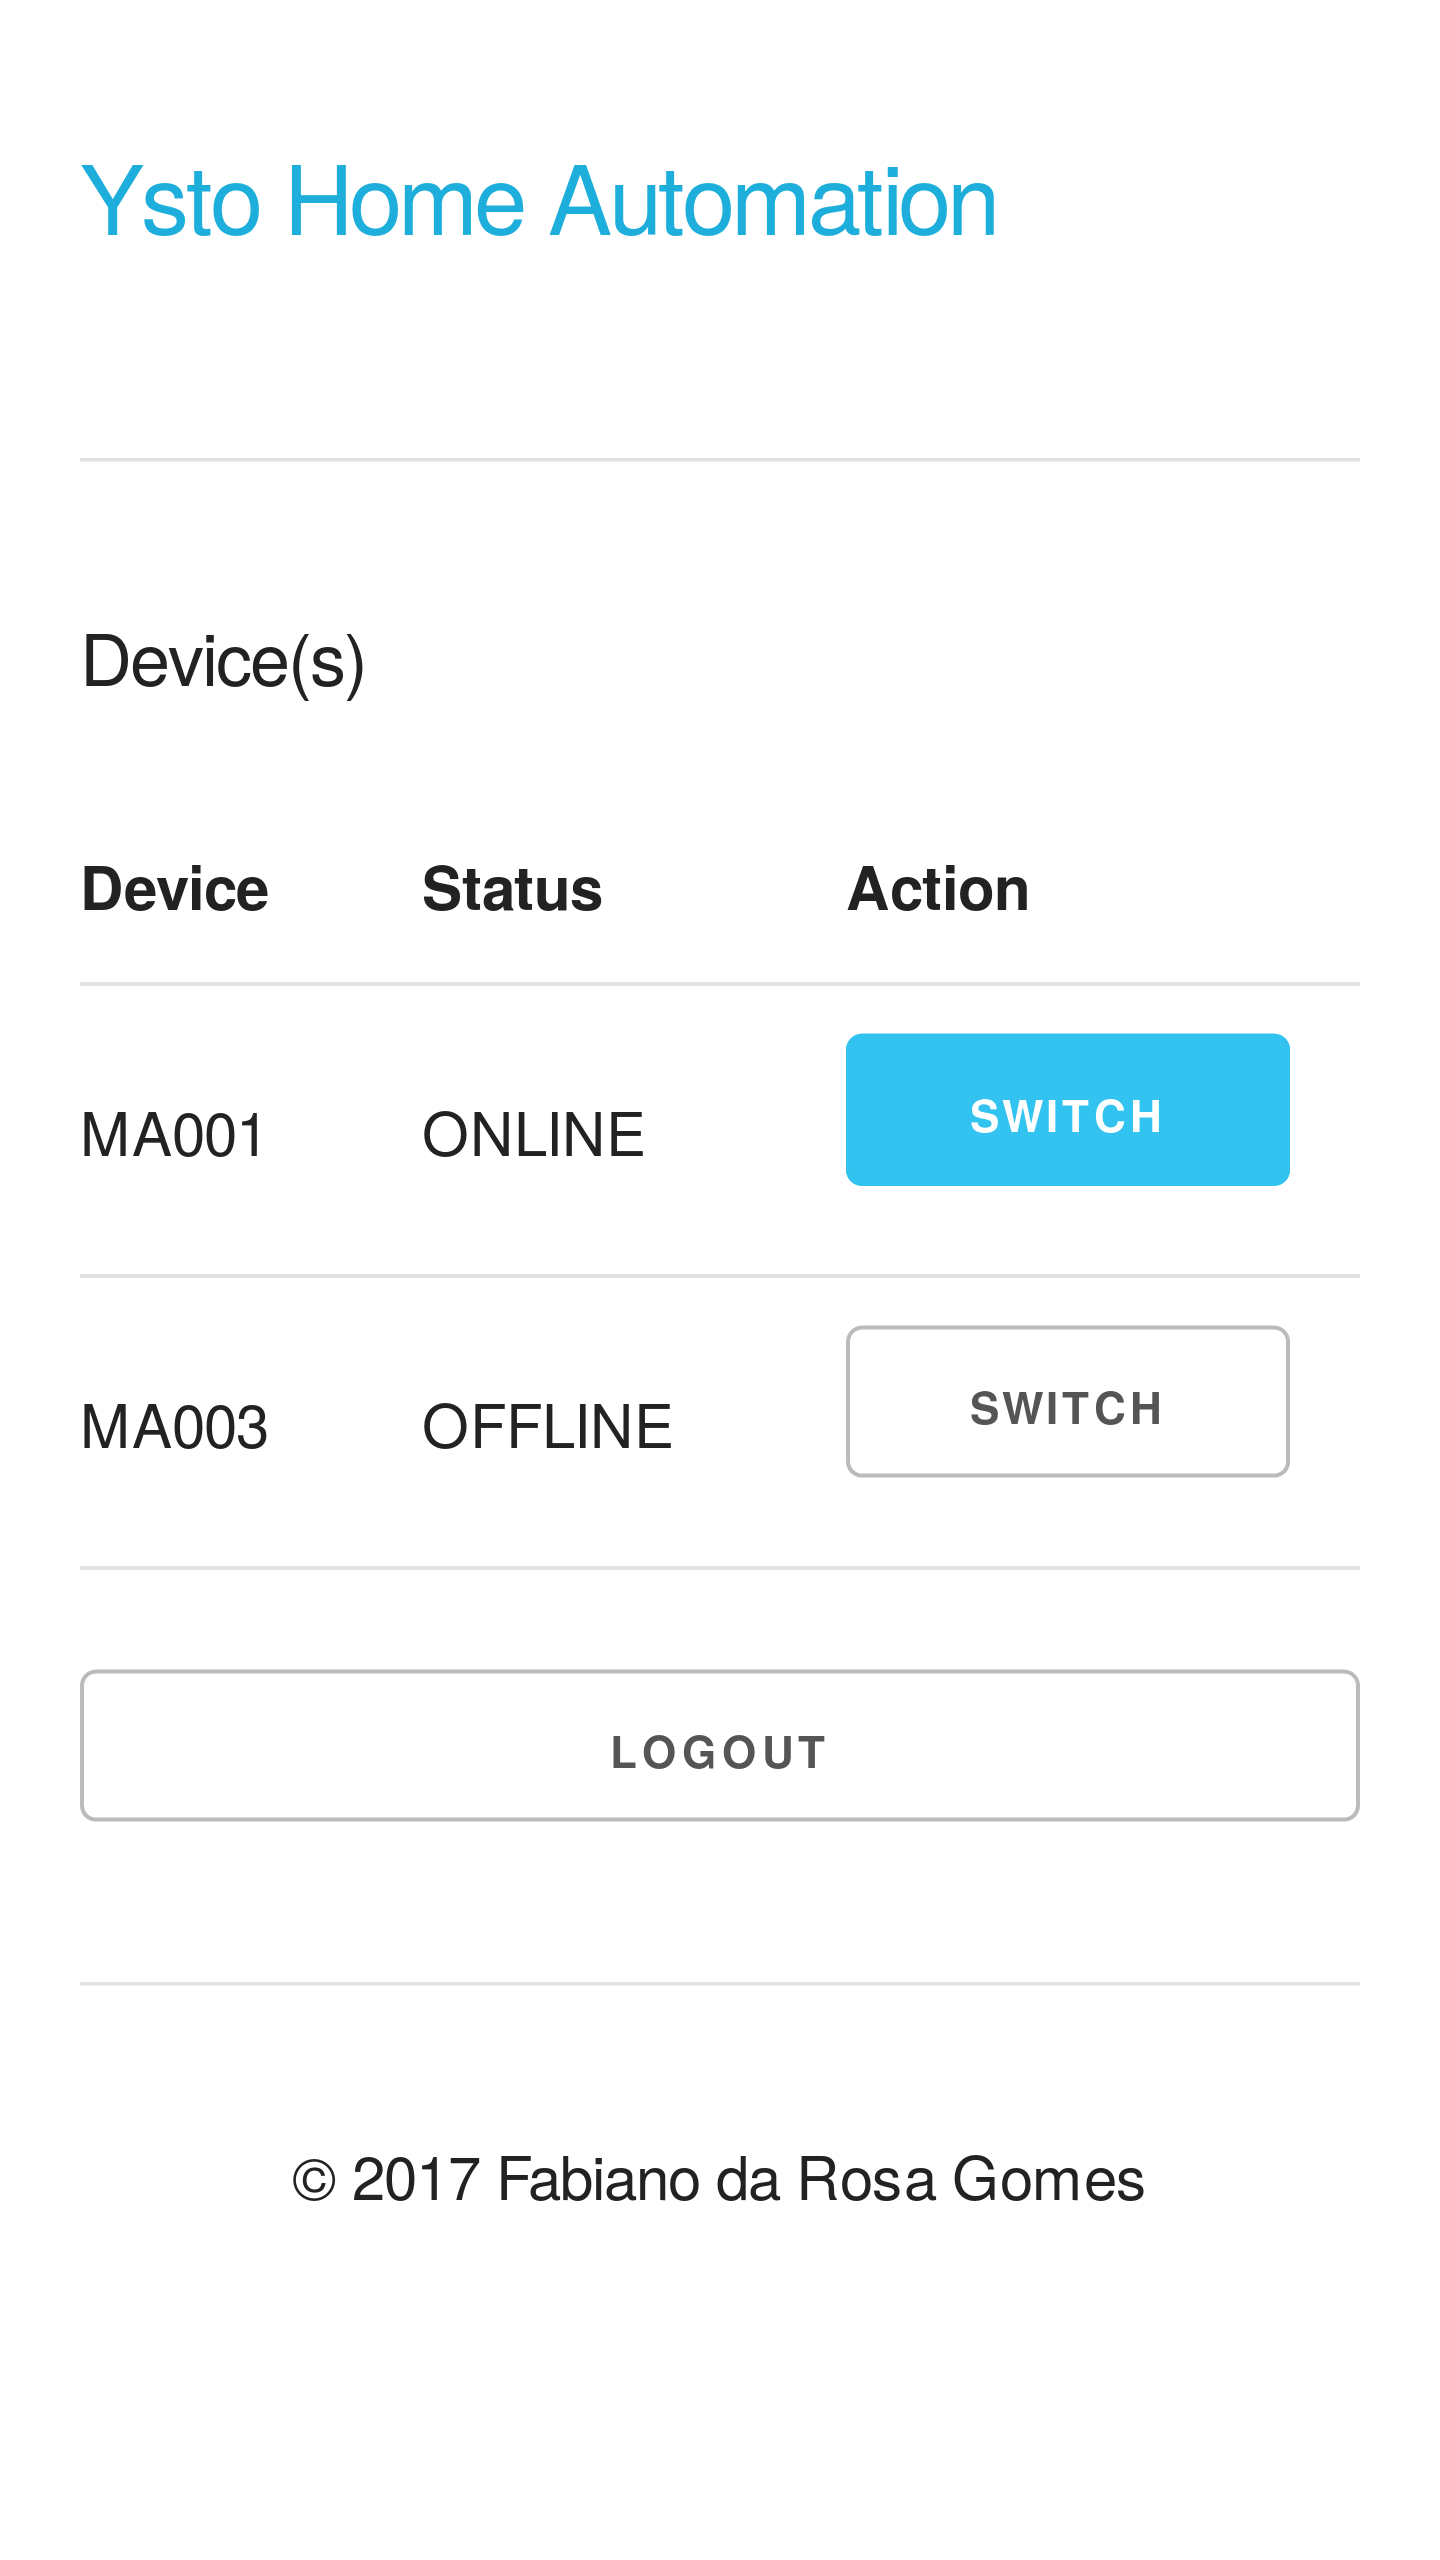
\includegraphics[scale=0.11]{img/04-device-control.png}}
\legend{Fonte: Autor do projeto}
\end{figure}

Por apresentar um \textit{layout} simples e com nome de funções de fácil entendimento, a utilização desta interface pretende oferecer um manuseio rápido e fácil mesmo para leigos no assunto.

\subsection{Retorno para tela inicial}
Para voltar para a tela de inicio, basta "clicar" no título da página de cada tela, no caso "Ysto Home Automation".
